\documentclass[12pt,a4paper,parskip=full]{scrartcl}

\usepackage{bbding}
\usepackage{pifont}
\usepackage{wasysym}
\usepackage[margin=1in]{geometry}
\geometry{letterpaper}
\usepackage{xcolor}
\definecolor{red}{HTML}{cc0000}
\definecolor{gray}{HTML}{666666}
\usepackage{sectsty}
\sectionfont{\color{red}}
\subsectionfont{\color{red}}
\subsubsectionfont{\color{red}}
\usepackage{graphicx}
\usepackage{hyperref}
\usepackage{amssymb}
\usepackage[style=footnote-dw]{biblatex}
\bibliography{S@SGuideBib}
\setlength\bibitemsep{0.5\baselineskip}
\graphicspath{{./images/}}

\usepackage{enumitem}
\setitemize{noitemsep}
% \setlist{noitemsep, topsep=-5pt}
% \setlength\itemsep{-0.10em}

\renewcommand{\labelitemi}{$\cdot$}
\renewcommand{\labelitemii}{$\cdot$}
\makeatletter
\let\latexl@section\l@section
\def\l@section#1#2{\begingroup\let\numberline\@gobble\latexl@section{#1}{#2}\endgroup}
\makeatother

\usepackage[T1]{fontenc}
\fontfamily{verdana}

\usepackage{scrlayer-scrpage}{}
\makeatletter
\renewcommand{\@seccntformat}[1]{}
\makeatother

\setlength\parindent{0pt}{}

\title{\Huge{\color{red}\textbf{The Scrum@Scale 
\textsuperscript{\copyright} 
Guide}}}
\subtitle{\color{gray}The Definitive Guide to Scrum@Scale:\\ Scaling that Works}
% \author{}
\date{}

\begin{document}

%\tableofcontents
%\newpage

\section{Purpose of the Scrum@Scale Guide}

Scrum, as originally outlined in the Scrum Guide, is a framework for developing, delivering, and sustaining complex products by a single team. Since its inception, its usage has extended to the creation of products, processes, services, and systems that require the efforts of multiple teams. Scrum@Scale was created to efficiently coordinate this new ecosystem of teams in a way that optimizes the overall strategy of the organization. It achieves this goal through setting up a ``minimum viable bureaucracy'' via a scale-free (below) architecture, which naturally extends the way a single Scrum Team functions across the organization.

This guide contains the definitions of the components that make up the Scrum@Scale framework, including its scaled roles, scaled events, and enterprise artifacts, as well as the rules that bind them together.

Dr. Jeff Sutherland developed Scrum@Scale based on the fundamental principles behind Scrum, Complex Adaptive Systems theory, game theory, and his work in biology. This guide was developed with the input of many experienced Scrum practitioners based on the results of their field work. 

\subsection{Why Scrum@Scale?}

Scrum was designed for a single team to be able to work at its optimal capacity while maintaining a sustainable pace. In the field, it was found that as the number of Scrum Teams within an organization grew, the output (working product) and velocity of those teams began to fall (due to issues like cross-team dependencies and duplication of work). It became obvious that a framework for effectively coordinating those teams was needed in order to achieve linear scalability. Scrum@Scale is designed to accomplish this goal via its scale-free architecture.

Scale-free architectures are commonly found in biological systems like the human body, and in chip design that requires putting billions of transistors on a chip. The internet is designed to be scale-free by every node having the same structure as every other node. By utilizing a scale-free architecture, an organization is not constrained to grow in a particular way determined by a set of arbitrary rules; rather it can grow organically based on its unique needs and at a sustainable pace of change that can be accepted by the groups of individuals that make up the organization. The simplicity of the Scrum@Scale model is essential to a scale-free architecture and carefully avoids introducing extra complexity that will cause productivity per team to decrease as more teams are created.

Scrum@Scale is designed to scale across the organization as a whole: all departments, products and services. It can be applied across multiple domains in all types of organizations in industry, government, or academia.  Scrum@Scale allows entire organizations to produce more valuable work at a faster yet sustainable cadence.

\subsection{Definition of Scrum@Scale}

\textbf{Scrum}: A framework within which people can address complex adaptive problems, while productively and creatively delivering viable products or services of the highest possible value.

The Scrum Guide is the minimal feature set that allows inspection and adaptability via radical transparency to drive innovation, customer satisfaction, performance, and team happiness.

\textbf{Scrum@Scale}: A framework for multiple Scrum Teams operating consistently with the Scrum Guide to address complex problems, while creatively delivering products or services of the highest possible value.
\textbf{NOTE}: These ``products'' may be hardware, software, complex integrated systems, processes, services, etc., depending upon the domain of the Scrum Teams.  These “services” may be customer support services, repair services, maintenance services, or government services.  

Scrum@Scale is:
\begin{itemize}
	\item Lightweight - the minimum viable bureaucracy
	\item Easy to understand - consists of only Scrum Teams
	\item Hard to master - requires implementing a new operating model
\end{itemize}

Scrum@Scale is a framework for scaling Scrum. It radically simplifies scaling by using Scrum to scale Scrum. 

Scrum@Scale consists of components that allow an organization to customize their transformational strategy and implementation. It gives them the ability to target their incrementally prioritized change efforts in the area(s) they deem most valuable or most in need of change and then progress on to others. 

In Scrum, the removal of impediments is a central component to increase team speed. In Scrum@Scale impediment removal is applied at scale to increase the speed of the entire organization.

In Scrum, care is taken to separate accountability of the ``what'' from the ``how.'' The same care is taken in Scrum@Scale so that jurisdiction and accountability are expressly understood in order to eliminate wasteful organizational conflict that keeps teams from achieving their optimal productivity.

In separating these two jurisdictions, Scrum@Scale contains two cycles: the Scrum Master Cycle (the ``how'') and the Product Owner Cycle (the ``what''), each touching the other at two points. Taken together, these cycles produce a powerful framework for coordinating the efforts of multiple teams along a single path.

Scrum@Scale can be applied when an organization has positions that match the Scrum roles. In other words, Scrum@Scale works if job titles such as Scrum Master and Product Owner define positions within an organization.  Scrum@Scale also works when positions do not match Scrum Roles. In such cases one may be hired to be a project manager (position) but may serve a Scrum Team as a Product Owner (role). There is no conflict between roles and positions. In agile organizations where roles (Scrum Master) and positions (regional manager) are not the same, great care should be taken to harmonize roles and positions. Harmonizing roles and positions can be as important to scaling Scrum as any other factor. Governance, roles, and positions should be aligned in any organization that has implemented Scrum to ensure that Scrum can scale and preserve both the speed of teams and the ability of teams to produce valuable products or services. Governance should address who has the authority to remove impediments.

\subsection{Values-Driven Culture}

Besides separating accountability of the ``what'' and the ``how,'' Scrum@Scale further aims to build healthy organizations by creating a values-driven culture in an empirical setting. The Scrum values are: Openness, Courage, Focus, Respect, and Commitment. These values drive empirical decision making, which depends on the three pillars of Transparency, Inspection, and Adaptation.

Openness supports Transparency into all of the work and processes, without which there is no ability to inspect them honestly and attempt to adapt them for the better. Courage refers to taking the bold leaps required to deliver value quicker in innovative ways.
Focus and Commitment refer to the way we handle our work obligations, putting customer value delivery as the highest priority. Lastly, all of this must occur in an environment based on Respect for the individuals doing the work, without whom nothing can be created.

Scrum@Scale helps organizations thrive by supporting a transformational leadership model which fosters a positive environment for working at a sustainable pace and putting commitment to deliver customer-facing value at the forefront of our efforts.

\subsection{The Components of the Scrum@Scale\textregistered ~Framework}

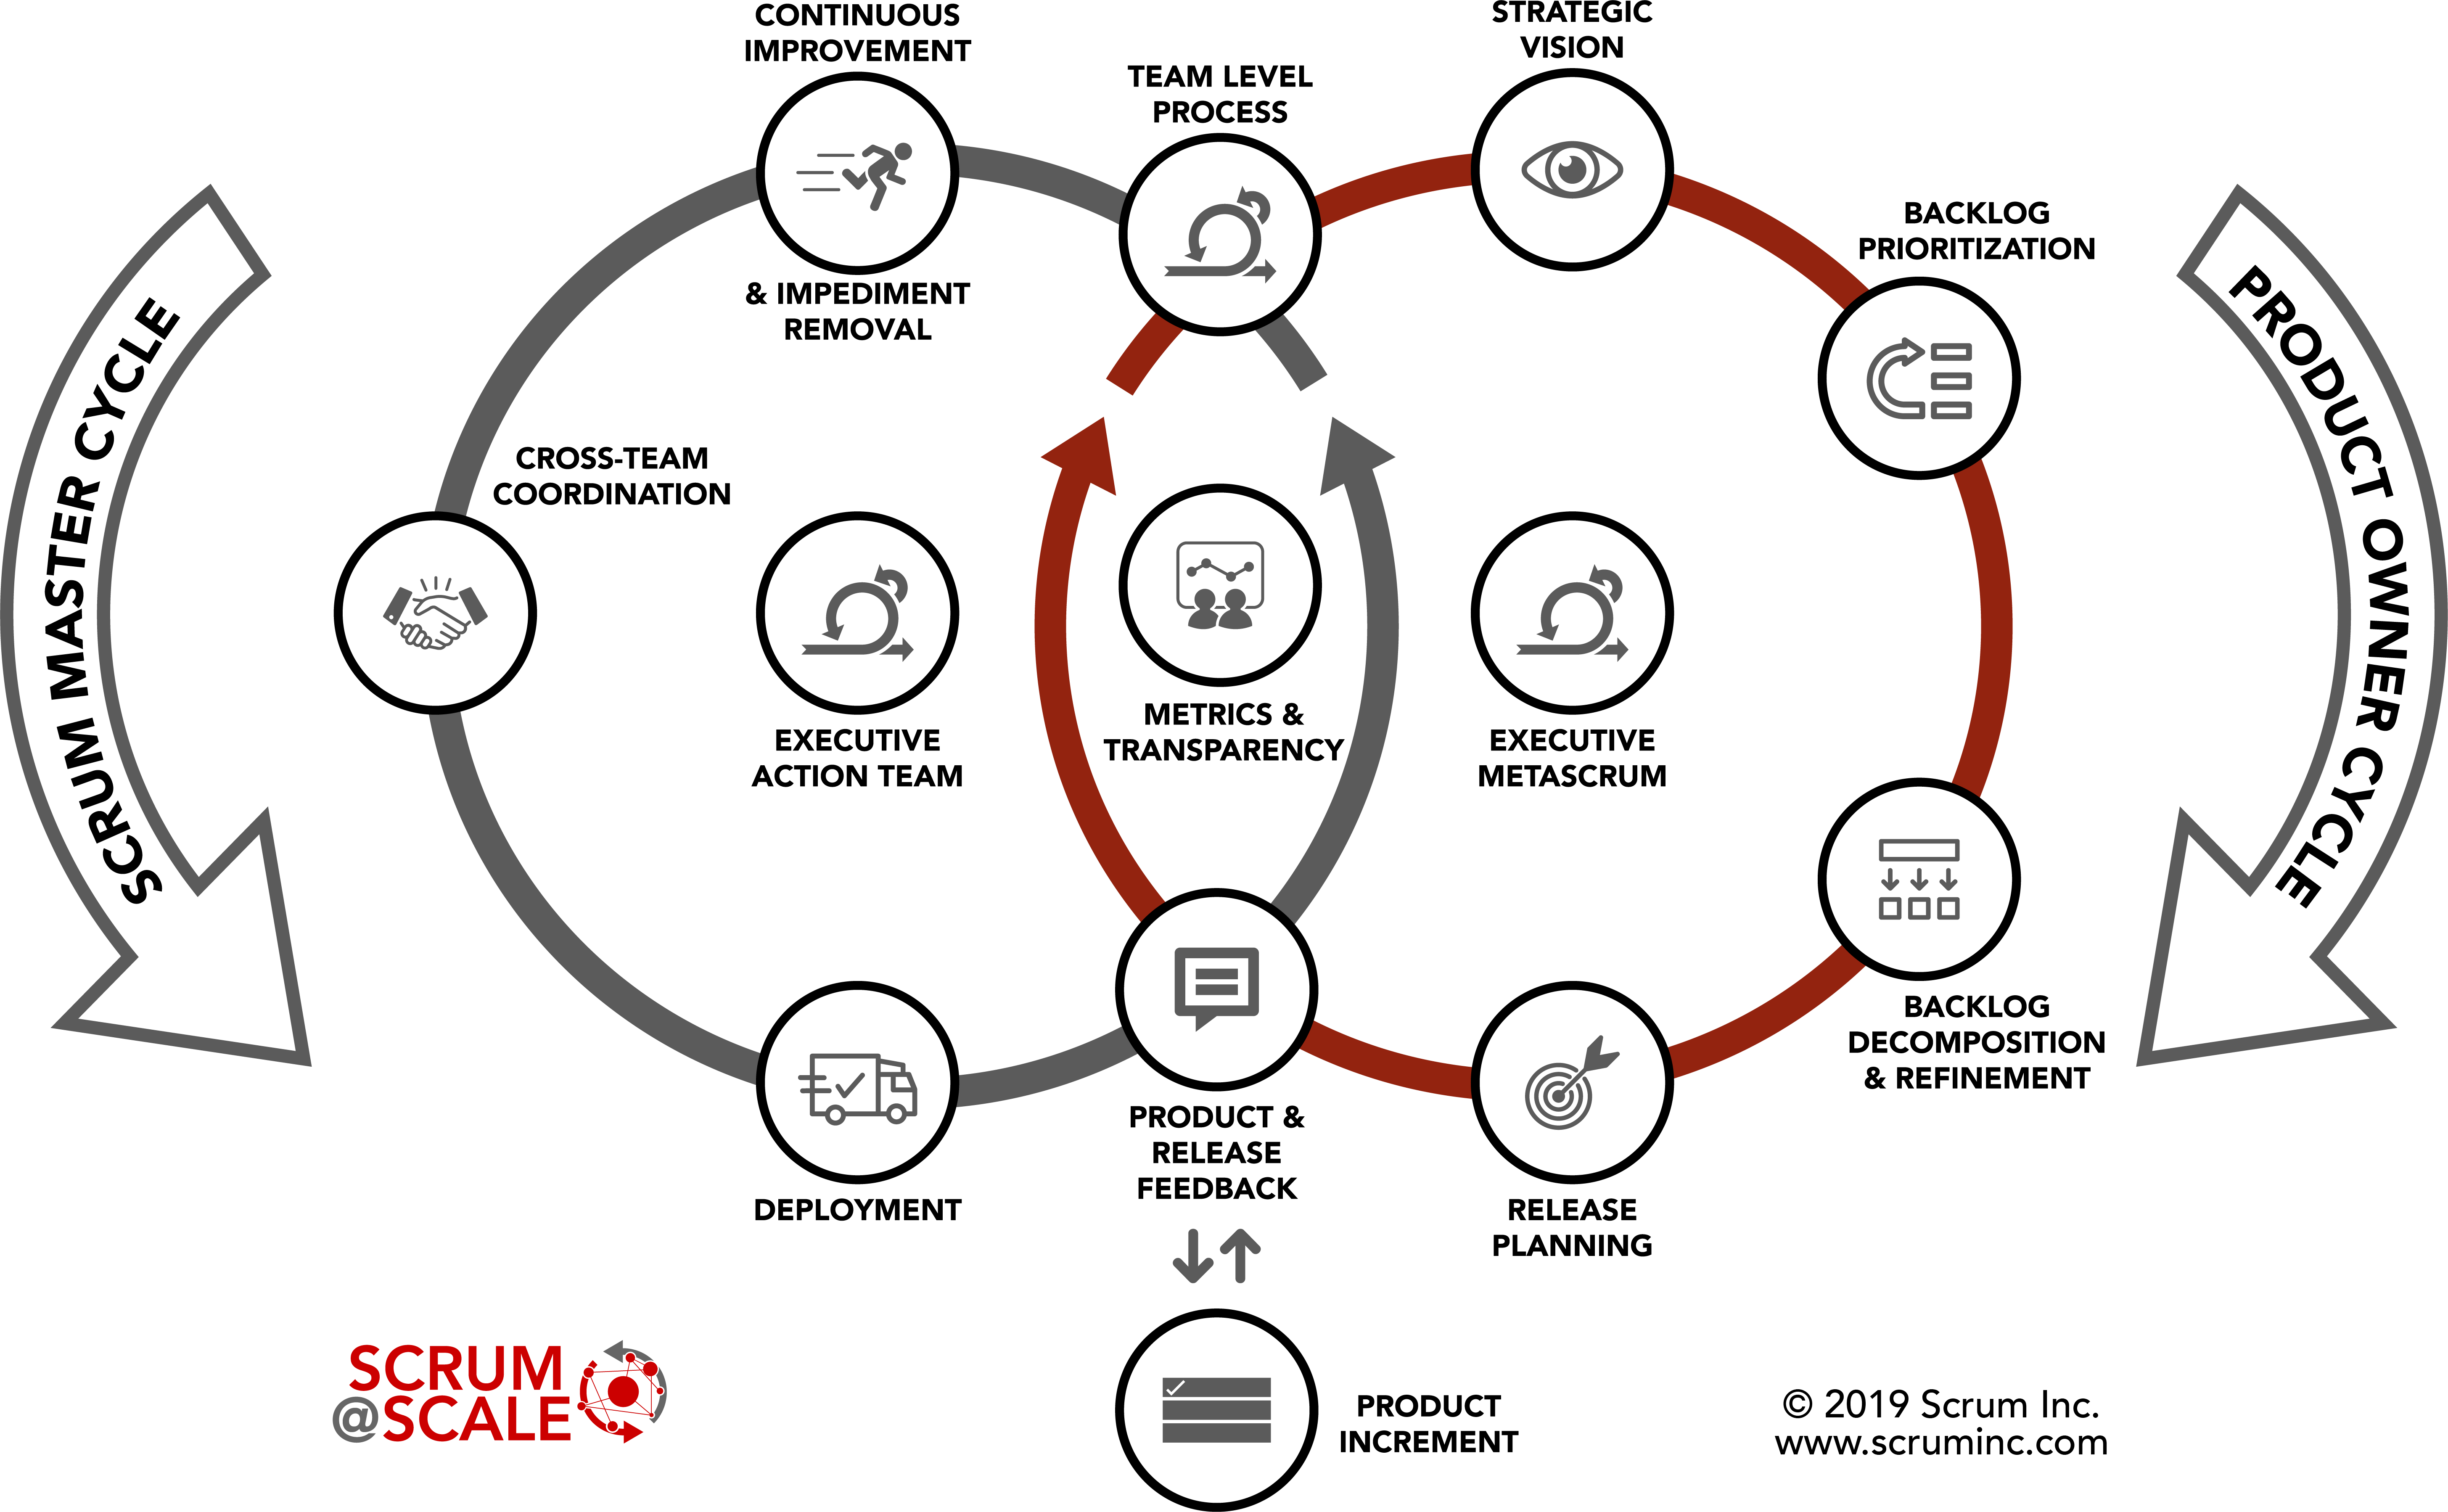
\includegraphics[width=1.0\linewidth]{SMPO-Cycle.png}

\section{Scaled Structure: the Scrum of Scrums}

A set of Scrum Teams that need to coordinate in order to deliver value to customers comprise a \textbf{Scrum of Scrums (SoS)}. This team is responsible for a fully integrated set of potentially shippable increments of product at the end of every Sprint from all participating teams. A SoS functions as a Release Team and must be able to directly deliver value to customers.

A Scrum of Scrums operates as a Scrum Team with scaled versions of the Scrum roles, events and artifacts. Given the scaled nature of the SoS there are some additional considerations.

\subsection{SoS Roles}

The SoS needs to have all of the skills necessary to deliver a fully integrated potentially shippable Product Increment at the end of every Sprint and to facilitate cross-team coordination where necessary. (It may need experienced architects, QA Leaders, members of the Product Ownership Team, and other operational skill sets.) 

\subsubsection{Product Owner Team}

For each SoS, there is an associated group of Product Owners called a \textbf{Product Owner Team} which aligns the teams' priorities along a single enterprise backlog so that they can coordinate their Scrum Team's backlogs and build alignment with stakeholders.

A team's Product Owner is responsible for the composition and prioritization of the team backlog and may pull backlog items from the shared SoS backlog into the team backlog or generate independent backlog items at their discretion.

The main functions of the Product Owner Team are to:

\begin{itemize}
	\item create an overarching vision for the product and make it visible to the organization.
	\item build alignment with key stakeholders to secure support for backlog implementation.
	\item generate a single, prioritized backlog, ensuring that duplication of work is avoided.
	\item assure impediments get resolved by properly prioritizing them in the backlog.
	\item create a minimal, uniform ``Definition of Done'' that applies to all teams.
	\item resolve dependencies raised by the teams.
	\item generate a coordinated Release Plan and forecast beyond the current Release Plan (often called a roadmap).
	\item decide upon and monitor metrics that give insight into the product and the market.
\end{itemize}

Product Owner Teams, just like SoS, function as Scrum Teams on their own. As such, they need to have someone acting as the Scrum Master and keeping the team on track in discussions. They also need a single person who is responsible for coordinating the generation of a single Product Backlog for all teams within the Scrum of Scrums. This person is designated as the \textbf{Chief Product Owner}.

\subsubsection{Chief Product Owner (CPO)}

The \textbf{Chief Product Owner} (CPO) coordinates priorities among Product Owners who work with individual teams. They align backlog priorities with Stakeholder and Customer needs. It may be an individual team PO who plays this role as well, or there may be a person specifically dedicated to this role. The responsibilities of the CPO are the same as that of a team PO, but at scale, the CPO is responsible for:

\begin{itemize}
	\item setting a strategic vision for the whole SoS.
	\item creating a single, prioritized backlog of value to be delivered by all of the teams.
	\begin{itemize}
		\item Note: these items are typically larger Product Backlog Items that will need further refinement and decomposition by the team POs.
	\end{itemize}
	\item working closely with their associated Scrum of Scrums Master (below) so that the Release Plan that the Product Owner team generates can be deployed efficiently.
	\item monitoring customer product feedback, as well as product feedback from the SoS, and adjusting the backlog accordingly.
	\item at the executive/meta level, leading the MetaScrum event where the overall Product Backlog is presented and alignment with stakeholders is achieved.
\end{itemize}



\subsubsection{Scrum of Scrums Master (SoSM)}

The Scrum Master of the Scrum of Scrums is called the \textbf{Scrum of Scrums Master (SoSM)}. The SoSM is accountable for the release of the joint teams' effort and must:

\begin{itemize}
	\item make progress visible.
	\item make an impediment backlog visible to the organization.
	\item remove impediments that the teams cannot address themselves.
	\item facilitate prioritization of impediments, with particular attention to cross-team dependencies and the distribution of backlog.
	\item improve the effectiveness of the Scrum of Scrums.
	\item work closely with the Product Owner Team to deploy a potentially releasable Product Increment at least every Sprint.
	\item coordinate the teams' deployment with the Product Owner's Release Plans.
\end{itemize}

\subsection{SoS Events}

\subsubsection{Scaled Daily Scrum (SDS)}

Since the SoS needs to be responsive to impediments raised by participating teams, at least one representative (usually the team's Scrum Master or whoever best understands the teams' impediment) of each of the participating teams needs to attend a \textbf{Scaled Daily Scrum (SDS)}. The SDS event mirrors the Daily Scrum in that it optimizes the collaboration and performance of the network of teams. Any person or number of people from participating teams may attend as needed. Additionally, the SDS:

\begin{itemize}
	\item is time-boxed to 15 minutes or less.
	\item must be attended by a representative of each team, including the Product Owner Team.
	\item is a forum where team representatives discuss what is going well, what is getting done, and how teams can work together more effectively. 
\end{itemize}
	
Some examples of what might be discussed are:
\begin{itemize}
	\item What impediments does my team have that will prevent them from accomplishing their Sprint Goal (or impact the upcoming release)?
	\item Is my team doing anything that will prevent another team from accomplishing their Sprint Goal (or impact their upcoming release)?
	\item Have we discovered any new dependencies between the teams or discovered a way to resolve an existing dependency?
	\item What improvements have we discovered that can be leveraged across teams?
\end{itemize}

\subsubsection{Dealing with Impediments in a SoS}


The SoSM should facilitate the refinement of an impediment backlog wherein impediments are identified as ``ready'' and prioritized to be removed. The teams then determine how best to remove them and how they will know when they are ``done.'' In some cases, impediment resolution may require product development, in which case, involvement from the SoS CPO and Product Owner Team will be necessary.


Particular attention should be paid to the SoS Retrospective in which the teams' representatives share any learnings or process improvements that their individual teams have succeeded with, in order to share best practices across the teams within the SoS.  

\section{Reference Model}

When implementing large networks of teams, it is critical to develop a scalable \textbf{Reference Model} for a small set of teams. Any deficiencies in a Scrum implementation will be magnified when multiple teams are deployed. Many of the initial scaling problems will be organizational policies and procedures or development practices that block high performance and frustrate teams. 

Therefore, the first challenge is to create a small set of teams that implements Scrum well.  This is best accomplished by the creation of an \textbf{Executive Action Team (EAT)} (below), which is accountable for the development and execution of the transformation strategy.  The EAT must be comprised of individuals who are empowered, politically and financially, to ensure the existence of the Reference Model. This set of teams works through organizational issues that block agility and creates a Reference Model for Scrum that is known to work in the organization and can be used as a pattern for scaling Scrum across the organization.

As the Reference Model of teams accelerates, impediments and bottlenecks that delay delivery, produce waste, or impede business agility become apparent. The most effective way to eliminate these problems is to spread Scrum across the organization so that the entire value stream is optimized.

Scrum@Scale achieves linear scaling in productivity by saturating the organization with Scrum and distributing velocity and quality organically, consistent with the organization's specific strategy, products, and services.

\section{Leadership Teams}

\subsection{Executive Action Team (EAT)}

The \textbf{Executive Action Team (EAT)} fulfills the Scrum Master role for the entire agile organization. This leadership team creates an agile bubble in the organization where the Reference Model operates with its own guidelines and procedures that integrates effectively with any part of the organization that is not agile. It owns the agile ecosystem, implements the Scrum values, and assures that Scrum roles are created and supported.

The EAT is the final stop for impediments that cannot be removed by the SoS that feed it. Therefore, it must be comprised of individuals who are empowered, politically and financially, to remove them. The function of the EAT is to coordinate multiple SoS and to interface with any non-agile parts of the organization. As with any Scrum Team, it needs a PO, a SM and a transparent backlog.

Sample Diagram showing an EAT coordinating 5 groupings of 25 teams:

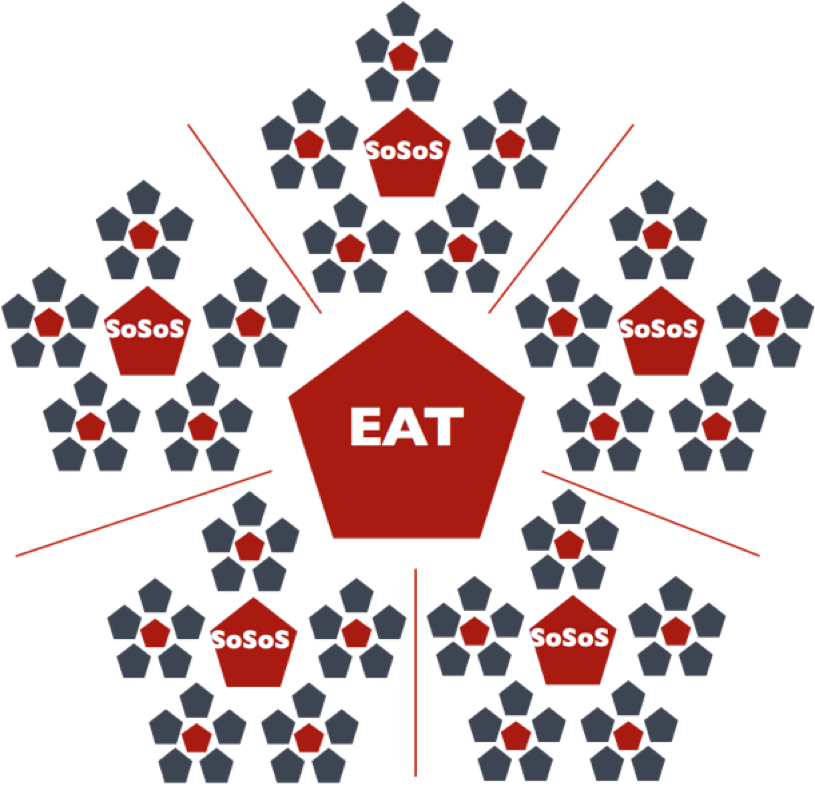
\includegraphics[width=\textwidth,height=\textheight,keepaspectratio]{SoS-EAT.png}

\subsubsection{EAT Backlog and Responsibilities}

The EAT is accountable for the quality of Scrum within the organization. As such, the entire SM organization reports to the EAT.

The EAT's role is to create an Organizational Transformation Backlog (a prioritized list of the agile initiatives that need to be accomplished) and see that it is carried out. The EAT ensures that a Product Owner organization is created and funded and that this organization is represented on the EAT to support these efforts. 

The EAT's responsibilities include but are not limited to:

\begin{itemize}
	\item creating an agile operating system for the Reference Model as it scales through the organization, including corporate operational rules, procedures, and guidelines to enable agility.
	\item measuring and improving the quality of Scrum in the organization.
	\item building capability within the organization for business agility.
	\item creating a center for continuous learning for Scrum professionals.
	\item supporting the exploration of new ways of working.
\end{itemize}

\subsection{Executive MetaScrum Team (EMT)}

The \textbf{Executive MetaScrum Team (EMT)} fulfills the Product Owner role for the entire agile organization. This leadership team owns the organizational vision and sets the strategic priorities, aligning all the teams around common goals. The Product Owner Teams enable a network design of Product Owners which is infinitely scalable with their associated SoS. The Product Owner Team for the entire agile organization meets with key stakeholders at the \textbf{MetaScrum Event} (below).

Sample diagram showing an EMT coordinating 5 groups of 25 teams:

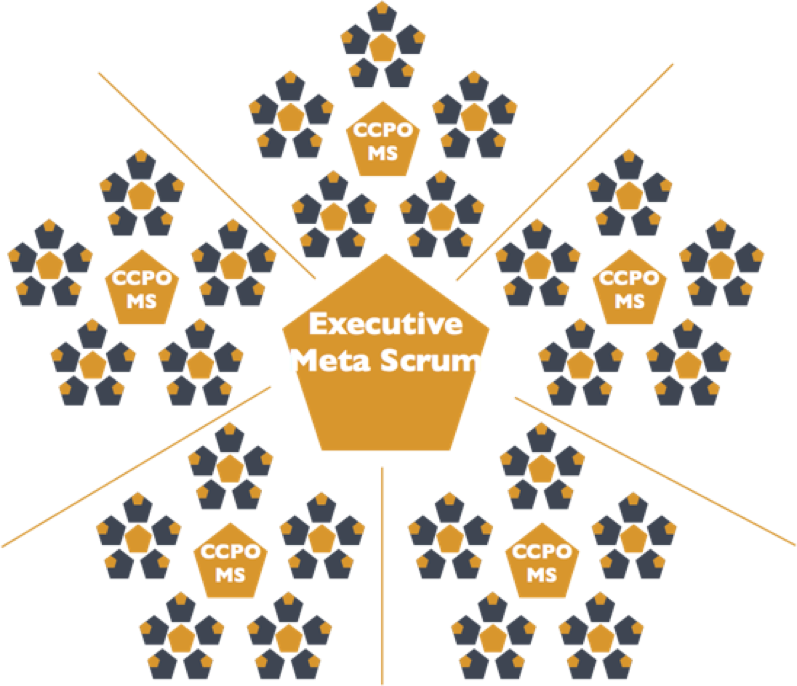
\includegraphics[width=1.0\linewidth]{ExecMetaScrum.png}

At least once per Sprint, the Executive MetaScrum Team holds a stakeholder alignment meeting, the \textbf{MetaScrum Event}. 

\begin{itemize}
	\item At the MetaScrum event, decisions affecting the entire organization get made. Changing direction of the organization, killing products and restructuring the organizational backlog can all happen at this event.
	\item The Chief Product Owner presents the Product Backlog to the MetaScrum Team, business owners who control funding, personnel, and customer commitments. They address any changes needed to strategy, funding, resource allocation, and deployments, and collaborate with the Chief Product Owner to build an agreement on a Product Backlog that they will support until the next MetaScrum Event.
\end{itemize}

\section{Scaling}

\subsection{Scaling the SoS}

Depending upon the size of the organization or implementation, more than one SoS may be needed to deliver a very complex product. In such cases, a \textbf{Scrum of Scrum of Scrums (SoSoS)} can be created out of multiple Scrums of Scrums. The SoSoS is an organic pattern of Scrum Teams which is infinitely scalable. Each SoSoS should have SoSoSMs and scaled versions of each artifact and event.

Scaling the SoS reduces the number of communication pathways within the organization so that complexity is encapsulated. The SoSoS interfaces with a SoS in the exact same manner that a SoS interfaces with a single Scrum Team, which allows for linear scalability.

Sample Diagrams:

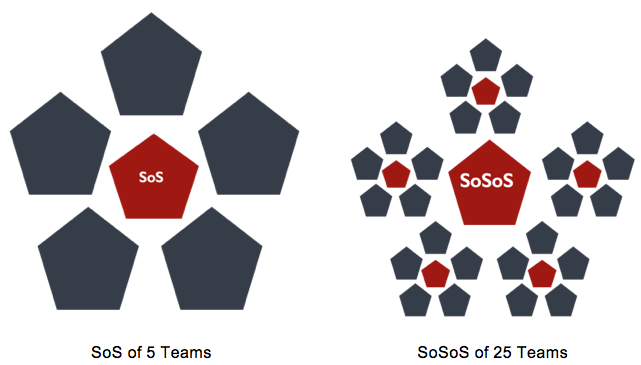
\includegraphics[width=1.0\linewidth]{Sos-R2.png}

\textbf{\textsc{note:}} While the Scrum Guide defines the optimal team size as being 3 to 9 people, Harvard research determined that optimal team size is 4.6 people (on average).\footnote{Hackman, J Richard, Leading teams: Setting the stage for great performances, Harvard Business Press, 2002} Experiments with high performing Scrum Teams have repeatedly shown that 4 or 5 people doing the work is the optimal size. It is essential to linear scalability that this pattern be the same for the number of teams in a SoS. Therefore, in the above and following diagrams, pentagons were chosen to represent a team of 5. These diagrams are meant to be examples only, your organizational diagram may differ greatly.

\subsection{Scaling the Product Owner Team}

Just as SoS can grow into SoSoS, Product Owner Teams also expand by the same mechanism. There is no specific term associated with these expanded units, nor do the CPO's of them have specific expanded titles. We encourage each organization to develop their own. For the following diagrams, we have chosen to add an additional ``Chief'' to the title of those PO's as they magnify out.

Sample diagrams:

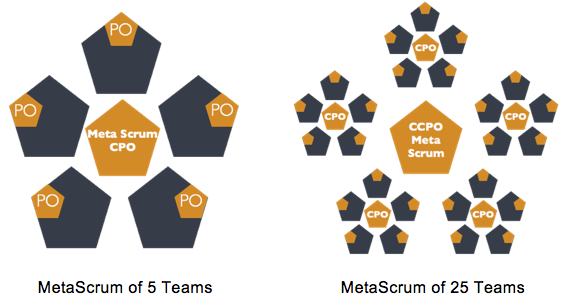
\includegraphics[width=1.0\linewidth]{MetaScrum-R2.png}

\section{Scrum Master Cycle - Coordinating the ``How''}

The SM organization (SM's, SoSM's, and EAT) work as a whole to complete the components of the Scrum Master Cycle. The components unique to the Scrum Master Cycle are: 
\begin{itemize}
	\item \textbf{Continuous Improvement and Impediment Removal},
	\item \textbf{Cross-Team Coordination}, and
	\item \textbf{Deployment}.
\end{itemize}

\subsection{Continuous Improvement and Impediment Removal}

In order to scale, impediments need to be removed as soon as possible.
Unresolved impediments scale with the implementation and cripple productivity.
We remove impediments to guarantee a scale-free architecture.

Continuous Improvement and Impediment Removal are repeatedly applied to:

\begin{itemize}
	\item identify impediments and reframe them as opportunities,
	\item ensure visibility in the organization to effect change,
	\item maintain a healthy and structured environment for prioritizing and removing impediments, and 
	\item verifying the resulting improvements.
\end{itemize}

\subsection{Cross-Team Coordination}

When multiple teams have to cooperate on the creation of a shared product,
they have a strong need to coordinate.

Cross-Team Coordination is essential in Scrum@Scale to:

\begin{itemize}
	\item coordinate similar processes across multiple related teams,
	\item mitigate cross-team dependencies to ensure they don't become impediments, and 
	\item maintain alignment of team norms and guidelines for consistent output.
\end{itemize}

\subsection{Deployment}

Since the goal of the SoS is to function as a release team, the deployment of product falls under their scope, while what is contained in any release falls under the scope of the Product Owners. Therefore, the goals of the Deployment are to:

\begin{itemize}
	\item deliver a consistent flow of valuable finished product to customers.
	\item integrate the work of different teams into one seamless product.
	\item ensure high quality of the customer experience.
\end{itemize}

\section{Product Owner Cycle - Coordinating the ``What''}

The PO organization (the Product Owners, the CPO's, and the Executive MetaScrum) work as a whole to satisfy the components of the Product Owner Cycle. The components unique to the Product Owner Cycle are:
\begin{itemize}
	\item \textbf{Strategic Vision},
	\item \textbf{Backlog Prioritization},
	\item \textbf{Backlog Decomposition and Refinement}, and
	\item \textbf{Release Planning}.
\end{itemize}

\subsection{Strategic Vision}

A compelling vision attracts both customers and great employees.
Therefore, in the PO cycle, a Strategic Vision needs to be formulated and communicated both internally and externally.

The goals of setting a Strategic Vision are to:

\begin{itemize}
	\item clearly align the entire organization along a shared path forward,
	\item compellingly articulate why the organization exists,
	\item describe what the organization will do to leverage key assets in support of its mission, and
	\item respond to rapidly changing market conditions.
\end{itemize}

\subsection{Backlog Prioritization}

Proper Prioritization Prevents Poor Performance.
Prioritizing the backlog can reveal activities that have negative value, no value or little value.
Identifying them and eliminating them provides focus and prevents waste.
Therefore, in Scrum@Scale, a crucial component of the PO cycle is Backlog Prioritization.

The goals of Backlog Prioritization are to:

\begin{itemize}
	\item identify a clear ordering for products, features, and services to be delivered;
	\item reflect value creation, risk mitigation and internal dependencies in ordering of the backlog, and
	\item prioritize the high-level initiatives across the entire agile organization prior to Backlog Decomposition and Refinement.
\end{itemize}

\subsection{Backlog Decomposition and Refinement}

Backlog gets pulled by teams.
In order for backlog from higher level teams to be pulled, it might need to be broken down and understood better.
This is done in the Backlog Decomposition and Refinement component of the PO cycle.

The goals of Backlog Decomposition and Refinement are to:

\begin{itemize}
	\item break complex products and projects into independent functional elements that can be completed by one team in one Sprint.
	\item capture and distill emerging requirements and customer feedback.
	\item ensure all backlog items are truly ``Ready'' so that they can be pulled by the individual teams.
\end{itemize}

\subsection{Release Planning}

The goals of Release Planning are to:

\begin{itemize}
	\item forecast delivery of key features and capabilities.
	\item communicate delivery expectations to stakeholders.
	\item update prioritization, as needed.
\end{itemize}

Note that Release Planning may encompass one or many releases of the product to a customer. It is a higher-level planning horizon than a single Sprint, usually covering a period of 1 to 6 months.

\section{Connecting the PO/SM Cycles}

The PO and SM Cycles have two touchpoints:
\begin{itemize}
	\item \textbf{Team-Level Process, and}
	\item \textbf{Product and Release Feedback.}
\end{itemize}
Both cycles need \textbf{Metrics and Transparency}.

\subsection{Team-Level Process}

The \textbf{Team-Level Process} is Scrum as prescribed by the Scrum Guide. It constitutes the first touch point between the Scrum Master and Product Owner Cycles. The goals of the Team-Level Process are to:

\begin{itemize}
	\item maximize the flow of completed and quality tested work.
	\item increase performance of the team over time.
	\item operate in a way that is sustainable and enriching for the team.
	\item accelerate the customer feedback loop.
\end{itemize}

\subsection{Product and Release Feedback}

The \textbf{Product and Release Feedback} component is the second point where the PO and SM Cycles touch. Product feedback drives continuous improvement through adjusting the Product Backlog while Release feedback drives continuous improvement through adjusting the Deployment mechanisms. The goals of obtaining and analyzing feedback are to:

\begin{itemize}
	\item validate our assumptions.
	\item understand how customers use and interact with the product.
	\item capture ideas for new features and functionality.
	\item define improvements to existing functionality.
	\item update progress towards product/project completion to refine release planning and stakeholder alignment.
	\item identify improvements to deployment methods and mechanisms.
\end{itemize}

\subsection{Metrics and Transparency}

Radical transparency is essential for Scrum to function optimally, but it is only possible in an organization that has embraced the Scrum values. It gives the organization the ability to honestly assess its progress and to inspect and adapt its products and processes. This is the foundation of the empirical nature of Scrum as laid out in the Scrum Guide.

Both the SM and PO Cycles require metrics that will be decided upon by the separate SM and PO organizations. Metrics may be unique to both specific organizations as well as to specific functions within those organizations. Scrum@Scale does not require any specific set of metrics, but it does suggest that at a bare minimum, the organization should measure:

\begin{itemize}
	\item Productivity - e.g. change in amount of Working Product delivered per Sprint
	\item Value Delivery - e.g. business value per unit of team effort
	\item Quality - e.g. defect rate or service downtime
	\item Sustainability - e.g. team happiness
\end{itemize}

The goals of having Metrics and Transparency are to:

\begin{itemize}
	\item provide all decision makers, including team members, with appropriate context to make good decisions.
	\item shorten feedback cycles as much as possible to avoid over-correction.
	\item require minimal additional effort by teams, stakeholders or leadership.
\end{itemize}

\section{Some notes on Organizational Design}

The scale-free nature of Scrum@Scale allows the design of the organization to be component-based, just like the framework itself. This permits for rebalancing or refactoring of teams in response to the market. As an organization grows, capturing the benefits of distributed teams may be important. Some organizations reach talent otherwise unavailable and are able to expand and contract as needed through outsourced development. Scrum@Scale enables linear scalability both in size and global distribution while avoiding long lag times, compromised communications, and inferior quality.\footnote{Sutherland, Jeff and Schoonheim, Guido and Rustenburg, Eelco and Rijk, Maurits, ``Fully distributed scrum: The secret sauce for hyperproductive offshored development teams'', AGILE'08. Conference, IEEE: 339-344, 2008}

Sample diagrams:
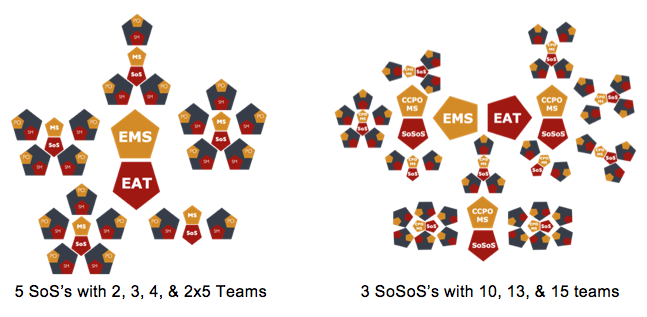
\includegraphics[width=1.0\linewidth]{VariableSoS-R2.png}
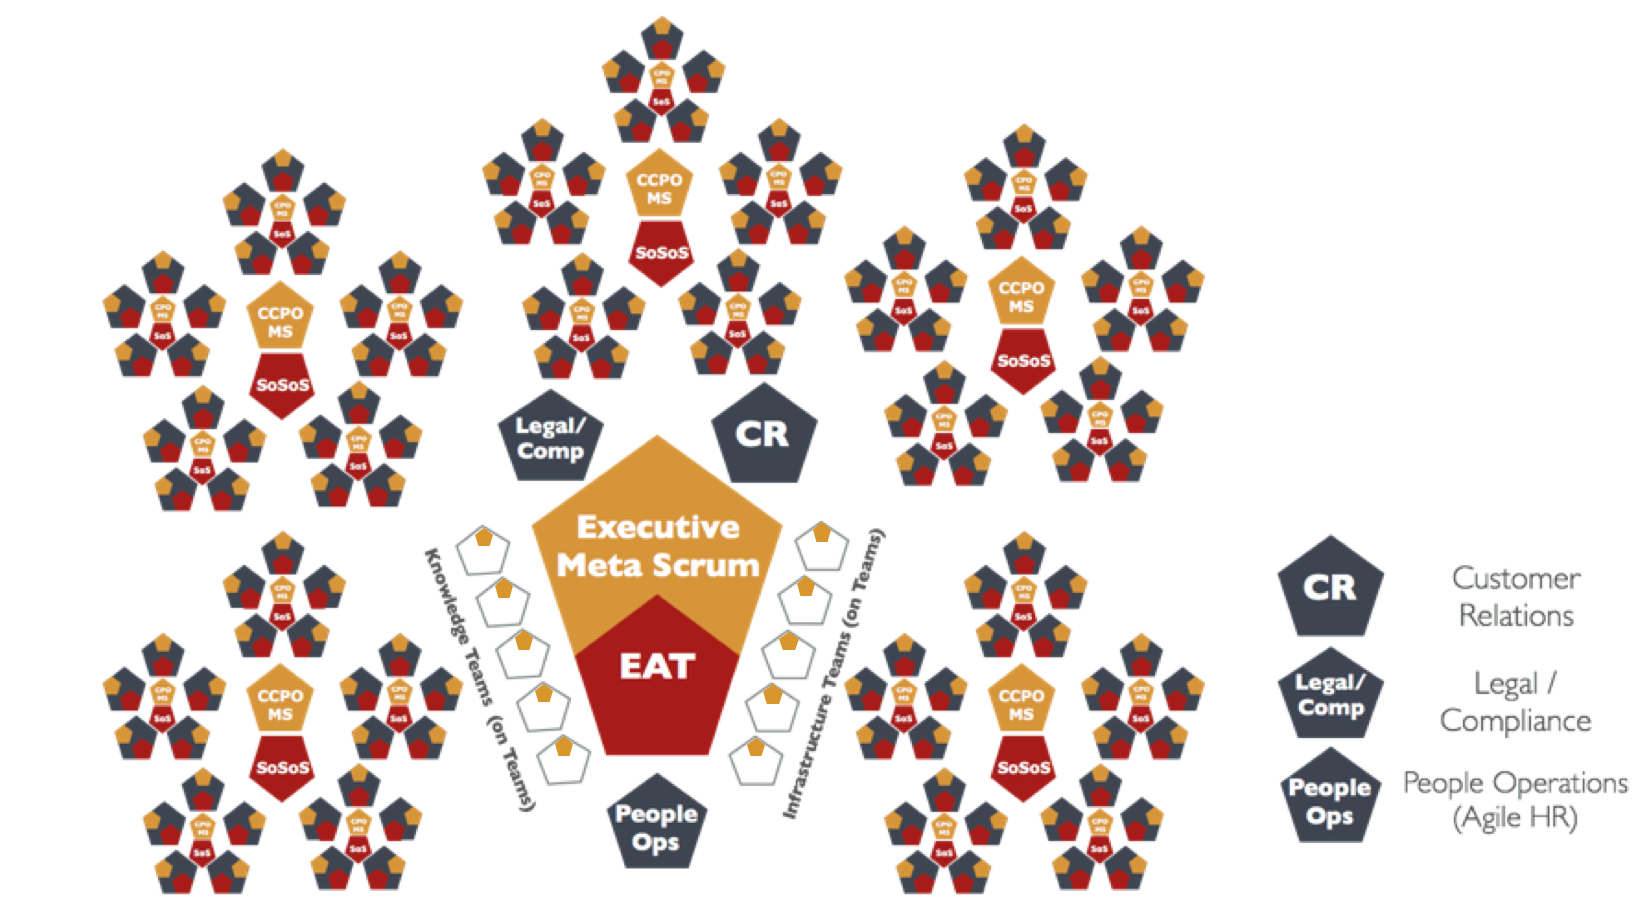
\includegraphics[width=1.0\linewidth]{OrganizationalDiagram.png}

In this organizational diagram, the \textbf{Knowledge and Infrastructure Teams} represent virtual teams of specialists of which there are too few to staff each team. They coordinate with the Scrum Teams as a group via service-level agreements where requests flow through a PO for each specialty who converts them into a transparent ordered backlog. An important note is that these teams are NOT silos of individuals who sit together (this is why they are represented as hollow pentagons); their team members sit on the actual Scrum Teams, but they make up this virtual Scrum of their own for the purpose of backlog dissemination and process improvement.

\textbf{Customer Relations, Legal / Compliance, and People Operations} are included here since they are necessary parts of organizations and will exist as independent Scrum Teams on their own, which all of the others may rely upon.

A final note on the representation of the EAT and EMT: in this diagram, they are shown as overlapping since some members sit on both of the teams. In very small organizations or implementations, the EAT and EMT may consist entirely of the same team members.

\section{End Note}

Scrum@Scale is designed to scale productivity, to get the entire organization delivering twice the value at half the cost in a significantly improved work environment. Large organizations that properly implement the framework can cut the cost of their products and services while improving quality and innovation.

Scrum@Scale is designed to saturate an organization with Scrum. All teams, including Leadership, Human Resources, Legal, Consulting and Training, and product and service teams, implement the same style of Scrum while streamlining and enhancing an organization.

Well implemented Scrum can run an entire organization and Scrum@Scale becomes the operating system for the organization.

\section{Acknowledgements}

We acknowledge IDX for the creation of the Scrum of Scrums which first allowed Scrum to scale to hundreds of teams,\footnote{Sutherland, Jeff, ``Inventing and Reinventing SCRUM in five Companies'', Sur le site officiel de l'alliance agile, 2001} PatientKeeper for the creation of the MetaScrum,\footnote{Sutherland, Jeff, ``Future of scrum: Parallel pipelining of sprints in complex projects'', Proceedings of the Agile Development Conference,  IEEE Computer Society 90-102,  2005.} which enabled rapid deployment of innovative product, and OpenView Venture Partners for scaling Scrum to the entire organization.\footnote{Sutherland, Jeff and Altman, Igor, ``Take no prisoners: How a venture capital group does scrum'', Agile Conference, 2009. AGILE'09, IEEE 350-355.  2009} We value input from Intel who taught us ``nothing scales'' except a scale-free architecture, and SAP with the largest Scrum team product organization who taught us management involvement in the MetaScrum is essential to get 2,000 Scrum Teams to work together.

The agile coaches and trainers implementing these concepts at Amazon, GE, 3M, Toyota, Spotify, Maersk, Comcast, AT\&T and many other companies working with Jeff Sutherland have been helpful in testing these concepts across a wide range of companies in different domains.

And finally, Avi Schneier, Alex Sutherland, Jessica Larsen, Kim Antelo, and Serge Beaumont have been invaluable in formulating and editing this document.

\pagebreak

\printbibliography

\end{document}
